\chapter{Introduction} \label{chapter_one}

Cameras have become an integral part of our lives. We use cameras regularly, be it a smartphone camera, a hobbyist camera setup or a professional camera. Our demand for high quality media from cameras is also increasing constantly. We want sharper, color accurate, low lighting bright photographs. The videos are expected to capture scenes with as much realism as possible and we don't want too many movements in them irrespective of the way we capture them. If we are making a video capturing a beautiful sunrise or a landscape while walking, we do not want movements associated with walking in our video. We want it to be as smooth as possible. This is where \textit{Video Stabilization} comes into play. Its goal being producing a stable video irrespective of the camera movements during capture.

% Motivation
\section{Motivation}

Image stabilization is a key technology to produce  good quality photographs and videos. Be it a 250,000 Euros television broadcast camera or a 100 Euros hobbyist camera, stabilization of some sort is necessary. That is why image stabilization exists in every camera and smartphone these days. There even exists a series of product lines from many big companies like DJI just for this specific reason; to stabilize the videos. These products can cost between less than 100 Euros for hobbyists to upwards of 1000 Euros or more for professionals. This clearly indicates that the need for stabilization is there and constant efforts are being put to make it better.

On microscopic level, the stabilization of videos becomes even more important as even small movements can cause large pixel shifts in the image plane. This can be seen by zooming in on your camera while trying to keep it stable. The effect of magnification becomes more evident and it will become increasingly more difficult to keep the video smooth and stable as the movements are magnified as well. This deteriorates the video quality and is very important to deal with. 

Microscopic movements are the scope of this work. A modified GoPro Hero 10 (Figure \ref{fig:mod_gopro_hero10}) camera is used as it allows to extract synchronized sensor and video data. The wide angle fisheye lens of the GoPro was exchanged with a narrow field-of-view lens that has a very large focal length. Switching the lens resulted in the default stabilization provided by GoPro (HyperSmooth) to not work anymore. The goal of this work is to explore different methods to obtain a stabilized video stream for large focal length lenses.

\begin{figure}[H]
    \centering
    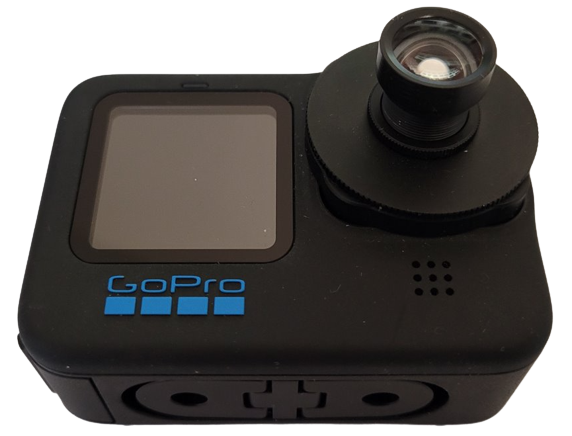
\includegraphics[scale=0.25]{images/fig_chapter4/mod_gorpro_hero_10.png}
    \caption{Modified GoPro Hero 10 with large focal length lens}
    \label{fig:mod_gopro_hero10}
\end{figure}


%\begin{itemize}
%\item Why am I doing this?
%\item Why is this relevant?
%\item What concrete problem do we want to solve?
%\item Is this problem big enough?

%\item Why is this exciting?
%\item What makes this problem challenging?
%\item Why an IMU Sensor? Why not just use Images?
%\end{itemize}

%How many times have to captured a video of something and when you looked at it later you found out that the video  is shaky? Image stabilization is inherent in producing good video quality. Be it a 250,000 Euro television broadcast camera or a 100 euro hobbyist camera, stabilization of some sort is necessary.


\section{Challenges}
We have a camera with small FOV high focal length lens which keeps vibrating on its rig. Vibrations are very small with a displacement of around 1.8mm but cause huge pixel shifts in the video recordings thus deteriorating the quality. Our goal is to stabilize the video so that there is no visual discomfort for the viewer and quality of the scene is preserved. We want to use an Inertial Measurement Unit (IMU) sensor to track these vibrations and stabilize the video based on it.

Noise is inherent to sensors and IMUs are no different. This presents a lot of challenges in accurate camera motion estimation. There exist IMU sensors with better noise characteristics, however, those are very expensive ($ > $1000 Euros) and are difficult to buy as they usually have a tactical grade placing them under export restrictions. Hence, in this work a low-cost consumer \textbf{MEMS} (Microelectromechanical systems) IMU is used. 

Use of IMUs for motion estimation for image stabilization presents many challenges including:

\begin{itemize}
    \item Accurate motion estimation over a longer period of time is not possible as the noise present in the readings results in \textbf{drift}.
    
    \item The drift is alleviated in translational motion estimation as it increases non-linearly with time.
    
    \item Working with drift is especially not possible in this case as we have an accuracy requirement of about 0.3 mm for the stabilization to work effectively.

    \item Classical algorithms fail to provide this accuracy over a long period of time as they are susceptible to strong drift without absolute pose updates which in this case is not possible.

    \item Due to these reasons, digital video stabilization using IMUs is rendered useless.
\end{itemize}
    
To deal with these challenges in other applications, IMUs are generally coupled with cameras, GPS and magnetometers to improve the accuracy but it is not possible for this use case. Irrespective of these pitfalls, the use of IMU is necessary for estimating these small motions. To tackle these challenges the following contributions are presented in this thesis:

\begin{itemize}
    \item Analysis of real motion characteristics and building a simulation based on that analysis to generate huge amount of data.

    \item As generating good data for data-driven approaches is very difficult, techniques for proper domain randomization are explored.

    \item Use of neural networks for accurate motion estimation using IMUs to combat drift.

    \item Exploring various neural network architectures that are able to learn motion characteristics of these vibrations.

    \item Development of a video stabilization pipeline using neural networks for motion estimation from IMU readings.
\end{itemize}


\subsubsection{Summary}
There are a lot of challenges in this work to overcome and end goal is important. That makes this work exciting. In the upcoming chapters, these challenges are discussed in detail and various solutions are explored. 

Chapter 2 includes the fundamental techniques and algorithms of video stabilization. It also entails the use and characteristics of IMUs for motion estimation. Pose estimation algorithms, including both classical and data driven, are also explored. Various neural networks architectures along with their possible use are investigated.

In chapter 3, state of the art algorithms for video stabilization and pose estimation are discussed. Chapter 4 examines the developed video stabilization pipeline and the measures taken to make it robust. Performance of various neural network architectures used is also evaluated.

Chapter 5 presents a brief overview of the techniques evaluated and the video stabilization pipeline developed. It concludes by discussing the future work required for further improvements and different applications.